%!TEX root = ../Thesis.tex
%\chapter{Introduction}
\chapter{Indledning}
Lægges en bold på en plan flade er der en god chance for der ikke går længe før denne triller af og ønsker man samtidig at kunne styre hvor på planen den rykker sig hen til og bliver kræver det at man konstant påvirker systemet. Stod med selv med planen i hænderne er det nemt at se hvordan man kan observere boldens position med sine øjne, bruge hjernen til at beslutte hvordan ens arme skal rykke og så rykke planen som får bolden til at flytte sig. Denne rutine forsætter man så med for at styre bolden rundt på planen. Dette kan selvfølgelig også gøres af en maskine. For at denne kan gøre dette kræves både en del matematik, elektronik og mekanik. En vigtig ting at sige om projektet er at selvom det har dele som kunne bruges til civile formål, har dette projekt til formål at fremvise elementer fra reguleringsteknik ved events som blandt andet åbent hus.

\section{Problemformulering}
Positionskontrol af en bold på en plan flade. Det er vigtigt at den er designet så den nemt kan bruges til åbnet hus event eller lignede. Desuden er det vigtigt at systemet er stabilt og har en homogen respons over hele fladen.
\clearpage
\section{Læringsmål for projektet}
\begin{itemize}
    \item kan arbejde selvstændigt og er i stand til at strukturere et større arbejde, herunder overholde tidsplaner og organisere og planlægge arbejdet
    \item kan sammenfatte og tolke teknisk information og behersker teknisk problemløsning gennem projektarbejde
    \item er i stand til at arbejde med alle faser i et projekt, herunder udarbejdelse af forslag, løsning og dokumentation
    \item er i stand til selvstændigt at tilegne sig ny viden og er desuden i stand til at forholde sig kritisk til tilegnet viden samt udføre relevant og kritisk informationssøgning og på den baggrund finde de rette metoder, til at belyse den aktuelle problemstilling.
    \item kan formidle teknisk information, teori og resultater skriftligt, visuelt/grafisk og mundtligt.
\end{itemize}
Dette projekt er gået fra idé, til planlægning til udførsel gennem redegørelse af problemet og derefter kortlægning af de delopgaver som skulle løses for at komme i mål. Det har været vigtigt at beslutte sig på forhånd hvad delmålene var og hvor længe de måtte tage at opnå.
Dette har betydet at en tidsplan er blevet fremstillet tidligt i forløbet, da man havde kortlagt de større arbejdsområder. Denne tidsplan er et arbejdsværktøj som skal sikre at man kommer igennem projekt og opnår hvad der er vigtigt uden at ende med at kæmpe for noget som kun giver mindre forbedringer.
Den berøringsfølsomme skræm brugt i projektet, havde ikke noget datasheet at finde, hvorfor jeg kontaktede fabrikanten, og udspurgte til produktet, herigennem fik jeg også nytte viden som kunne bruge i delen om dataindsamling. Da produktet typisk bliver brugt med en færdig lavet kontroller, var disse datasheets en god kilde til inspiration, hvorfor disse også er angivet som kilder. 
Dette projekt indeholder både en elektrisk del, samt design af en mekanik. Der er klart været mere fokus på den elektriske del, især styringen, mens det meste af det mekaniske er der blevet fremstillet ved hjælp af 3d print.
Da der er mange mindre dele i projektet og hver især bør dokumenters til forskellige detalje grader ud fra en prioritering af tid, er det vigtigt at man indsamler data når man laver den, og giver den fornuftige navne så disse kan bruge til god dokumentation som ligger til baggrund for ens beslutninger i design fasen.
For at samle op på alle resultater, beslutninger og analyser er det også vigtigt at skrive en rapport som sørge for at gøre det klart for læseren hvordan og hvorfor man har udført arbejdet på lige den måde.
\clearpage
\section{Liste af opgaver med beskrivelse og tidsforbrug}
\begin{itemize}
\item	Matematisk model (4 uger)
\\	Systemet indeholder elektriske dele såvel som mekaniske, disse skal beskrives i en passende detalje grad så kontrolleren kan tunes og implementeres.
Det er vigtigt ikke at tage unødige ting med, men samtidige sørge for at ens model og virkeligheden ligner hinanden tilfredsstillende så ens kontroller ikke kun virker teoretisk.
\item	Kontroller design (4 uger)
\\	Der vil ud fra den matematiske model blive beregnet en lineær overføringsfunktion som jeg ved hjælp af en frekvensanalyse vil designe min kontroller med. Det er vigtigt at denne ikke giver anledning til unødige svingninger og rystelser i den mekaniske konstruktion samtidige med at den ikke må være for langsom og ude af stand til at styre boldens position.
\item	Mekaniske konstruktion til både motor, microcontroller og trykfølsomoverfalde (4 uger)
\\	Denne skal bestå af en holder til pladen som tillader bevægelse i både x og y retningen. Her er det desuden vigtigt at tænke ind at man nemt bør kunne bære konstruktionen så denne kan medbringes til åbent hus.
\item	Motor styring (2 uger)
\\	Da microcontrolleren valgt at bruge ikke selv kan kører motorne er det vigtigt at disse får strøm andet sted fra, dette skal bygges op, men ud fra hensyn om at minimere omfanget af projektet som helhed, så det nemmere kan bruges til åbent hus.
\item	UI (1 uge)
\\	Der skal bygges et brugerinterface op så det er muligt at vælge hvad funktion der udføres, såsom gå til midten af pladen eller kør i en firkant. Her tænkes at bruge knapper og LED lys, så det er simpelt at følge med i hvad funktion som er valgt og vælge en ny.
\item	Kontroller implementering (5 uger)
\\	Der skal kodes både funktioner for aflæsning af værdier, beregningen af nye motor variabler samt valg af ønsket mønster.
\\	Dette deler koden op i tre dele.
\\	En del som handler om aflæsning, en del som handler om styring, samt en del som handler om brugerflade.
\\	Aflæsningen af data fra sensoren skal ske så man ender op med kun at arbejde med data som ikke indeholder for meget støj.
\\	Det er vigtigt at fokus lægges på de to første dele, da disse er dele af styringskredsen.
\item	Rapport skrivning (8 uger)
\\	Der skal skrives afsnit om alle de større emner som blandt andet se nogle af foroven. Det er vigtigt at man løbende skriver og arbejder med dokumentationen og fremvisningen af ens resultater.



\end{itemize}

\clearpage
\section{Tidsplan - Gantt-skema}
\begin{figure}[!h]
\centering
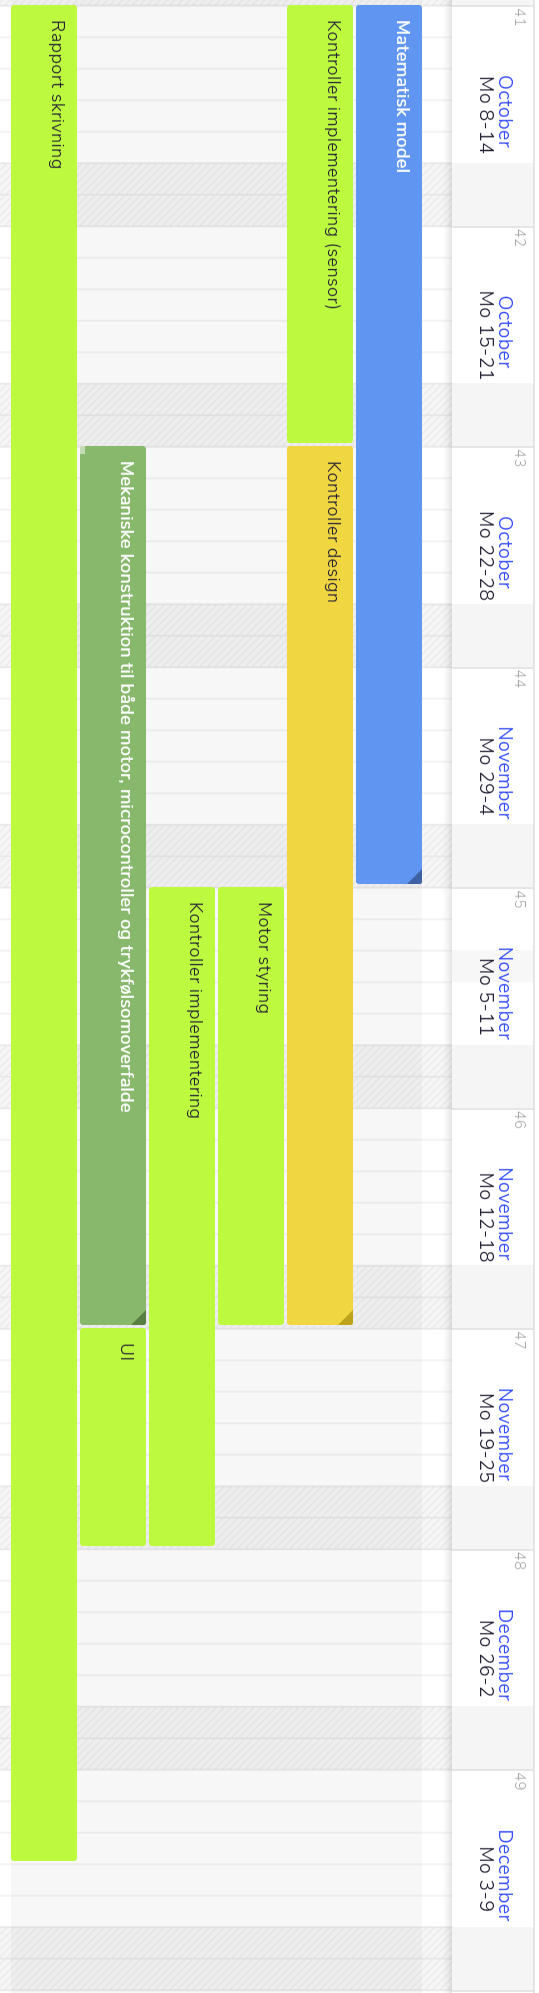
\includegraphics[scale=0.55]{Capture2}
\caption{Gantt-skema}
\label{FIG:DTULOGO}
\end{figure}